%\documentclass[12pt]{report}
%\author{Emmanuel Bency, Priyabrata Majhi}
%\date{}
%\usepackage{../sem12-lab-record}
\lhead{Date: 23/07/2021}  % For date in header

% REMOVE the % sign in the above lines if you want to
% compile this experiment file separately.

\begin{document}
	
	\chapter{Fermi Energy of Copper} % Replace the text with the title of the experiment
	\vspace{-1cm}
	\dateofexp{Date of Experiment: 23/07/2021}
	% To display date in contents page
	
	\begin{center}% To display date of experiment in the title
		Date of Experiment: 23/07/2021
	\end{center}
	
	%%%%%%%%%%%%%%%%%%%%%%%%%%%%%%%%%%%%%%%%%%%%%
	% THE EXPERIMENT STARTS HERE %
	%%%%%%%%%%%%%%%%%%%%%%%%%%%%%%%%%%%%%%%%%%%%%
	
	\section{Aim}
	To determine the Fermi energy of Copper and hence to calculate the mean free path and relaxation time.
	
	\section{Requirements}
	\begin{itemize}
		\item 	Copper wire
		\item 	Electric stove
		\item   Beaker
		\item   Digital thermometer
		\item   Digital multimeter
		\item   Paraffin
	\end{itemize}
	
	\section{Theory}
	Free electrons in metals and semiconductors can be approximately considered as behaving like a gas (Fermi gas). The energy distribution of the fermions in a Fermi gas in thermal equilibrium is determined by their density, the temperature and the set of available energy states using Fermi-Dirac statistics. The distribution of electrons according to this statistics implies that at 0K, the electors occupy all the lower energy levels subject to Pauli exclusion principle. The energy of the top most filled level at 0K is called the Fermi energy $E_{f}$. At other temperatures this is the energy of that level whose probability of occupation is $1/2$. At temperatures greater than \SI{0}{\kelvin}, the thermal energy available to the electrons is capable of causing only those small fraction of electrons lying below the Fermi level to reach higher levels. As a result, the contribution of electrons to the electrical and thermal conductivities is relatively small.
	
	The number $n$ of free electrons in metal per unit volume is given by, 
	\begin{equation}\label{eqn:n}
		n=\dfrac{N \rho}{M}
	\end{equation}
	where $N = \SI{6.023E26}{\per\meter\cubed}$ is the Avogadro number, $\rho,\, M$ are the density and mass number of the metal. Suppose $L, A$ are the length and cross sectional area of the metal in the form of a wire whose resistance is $R$, then the electrical conductivity $\sigma$ of the metal is:
	\begin{equation}\label{eqn:sigma-1}
		\sigma=\dfrac{L}{RA}
	\end{equation}

	$\Theta$, the \emph{Debye temperature}, is the characteristic temperature of the thermal vibrations of the crystal lattice. For temperatures much higher than $\Theta$, $\sigma \propto 1/T$. 
	If $\tau_{F}$ is the mean relaxation time of the electrons, then the conductivity is given by the more general form
	\begin{equation}{\label{eqn:condeqn}}
		\sigma=\frac{n e^{2} \tau_{F}}{m} 
	\end{equation}
	where $m$ is the mass of the electron. The Fermi velocity of electron is expressed in terms of mean free path $\lambda_{F}$, and relaxation time $\tau_{F}$ as,
	\begin{equation}\label{eqn:Fermi-velocity}
		v_F = \frac{\lambda_{F}}{\tau_F}   
	\end{equation}
	Thus the Fermi energy is expressed as
	\begin{equation}\label{eqn:FermiEnergy1}
		E_{F}=\frac{m\lambda_{F}^2}{2\tau_{F}^2}   
	\end{equation}
	Now,equation(\ref{eqn:condeqn}) can be utilized to get Fermi energy as,
	\begin{equation}\label{eqn:FermiEnergy2}
		E_{F}= \left(\frac{ne^2\lambda_{F}R\pi r^2}{L\sqrt{2m}}\right)^2   
	\end{equation} 
	where conductivity, $\sigma=L/{R\pi r^2}$, with $L$ as the length of the copper wire, $r$ as the radius of the wire and $R$, the resistance of the wire utilized.
	
	The above formula can be rewritten, to include temperature dependence of resistance of copper as
	\begin{equation}{\label{eqn:FermiEnergy-MAIN}}
		E_{F}=\left(\frac{ne^2\pi Ar^2}{L\sqrt{2m}}\right)^2 \times \left(\dfrac{\Delta R}{\Delta T}\right)^2 \text{joules}
	\end{equation}
	where, $n=\SI{8.5e28}{\per\meter\cubed}$ \\
	$e=\SI{1.6E-19}{\coulomb}$ \\
	$A=9.8\times 10^{-6}$ \\
	$m=9.1\times 10^{-31}$kg \\
	Radius of the wire ($ r $)= $0.014\times 10^{-2}$ m.\\
	Length of the wire ($ L $)= 15 m\\
	$\left(\dfrac{\Delta R}{\Delta T}\right)$=Slope of R vs T graph.
	
	The first term in the above equation is a constant, which is evaluated to be \SI{4.23E-15}{}. So the formula reduces to :
	\begin{equation}{\label{eqn:FermiEnergy-REDUCED}}
		\boxed{E_{F}=\left(4.23\times10^{-15}\right) \times \left(\text{slope of } R-T \text{ graph}\right)^2} \quad \text{joules}
	\end{equation}
	
	Once $E_{f}$ is found out, the Fermi speed $v_{f}$, the relaxation time and mean free path are calculated using
	\begin{equation}\label{eqn:Fermi-velocity-MAIN}
		v_{F}=\sqrt{\frac{2 E_{F}}{m}}=1.482 \times 10^{15} \sqrt{E_{F}} \, \si{\meter\per\second}
	\end{equation}
	\begin{equation}\label{eqn:tau-F-MAIN}
		\tau_{F}=\frac{\sigma m}{ne^{2}}=\frac{m}{ne^{2}\rho}
	\end{equation}
	\begin{equation}\label{eqn:lambda-F-MAIN}
		\lambda_{F}=v_{F}\tau_{F} 
	\end{equation}
	
	\section{Procedure}
	
	\begin{enumerate}
		\item 	Copper wire is wound on an insulator and is dipped in an oil bath.
		\item 	 A \SI{0}{\degreeCelsius}-\SI{200}{\degreeCelsius} thermometer is used to measure the temperature of the oil in the bath.
		\item 	 The resistance of the wire is determined at various temperatures using a sensitive ohmmeter during the cooling phase.
		\item  	The oil bath should not be heated to above \SI{120}{\degreeCelsius}, to avoid the possibility of the copper wire breaking.
	\end{enumerate}
	
	\begin{figure}[H]
		\centering
		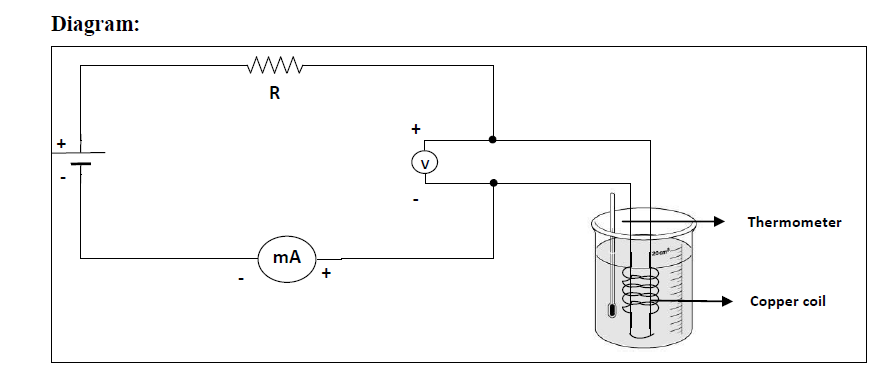
\includegraphics[width=\textwidth]{Experiments/Ch-05-diagram.png}
		\caption{Circuit Diagram}
		\label{fig:1205-diagram}	
	\end{figure}
	
	\section{Observations \& Graph}
	
		\begin{longtable}{|r|r|r|}
			\hline
			\rowcolor[HTML]{EFEFEF} 
			\multicolumn{1}{|c|}{\cellcolor[HTML]{EFEFEF}\begin{tabular}[c]{@{}c@{}}Temperature\\ (\si{\degreeCelsius})\end{tabular}} & \multicolumn{1}{c|}{\cellcolor[HTML]{EFEFEF}\begin{tabular}[c]{@{}c@{}}Temperature\\ (\si{\kelvin})\end{tabular}} & \multicolumn{1}{c|}{\cellcolor[HTML]{EFEFEF}\begin{tabular}[c]{@{}c@{}}Resistance\\ (\si{\ohm})\end{tabular}} \\ \hline
			130                                                                                                     & 403.15                                                                                                 & 4.9                                                                                                  \\ \hline
			125                                                                                                     & 398.15                                                                                                 & 4.8                                                                                                  \\ \hline
			120                                                                                                     & 393.15                                                                                                 & 4.8                                                                                                  \\ \hline
			115                                                                                                     & 388.15                                                                                                 & 4.8                                                                                                  \\ \hline
			110                                                                                                     & 383.15                                                                                                 & 4.7                                                                                                  \\ \hline
			105                                                                                                     & 378.15                                                                                                 & 4.7                                                                                                  \\ \hline
			100                                                                                                     & 373.15                                                                                                 & 4.6                                                                                                  \\ \hline
			95                                                                                                      & 368.15                                                                                                 & 4.5                                                                                                  \\ \hline
			90                                                                                                      & 363.15                                                                                                 & 4.5                                                                                                  \\ \hline
			85                                                                                                      & 358.15                                                                                                 & 4.4                                                                                                  \\ \hline
			80                                                                                                      & 353.15                                                                                                 & 4.3                                                                                                  \\ \hline
			75                                                                                                      & 348.15                                                                                                 & 4.3                                                                                                  \\ \hline
			70                                                                                                      & 343.15                                                                                                 & 4.2                                                                                                  \\ \hline
			65                                                                                                      & 338.15                                                                                                 & 4.1                                                                                                  \\ \hline
			60                                                                                                      & 333.15                                                                                                 & 4.1                                                                                                  \\ \hline
			55                                                                                                      & 328.15                                                                                                 & 4.0                                                                                                  \\ \hline
			50                                                                                                      & 323.15                                                                                                 & 3.9                                                                                                  \\ \hline
			45                                                                                                      & 318.15                                                                                                 & 3.8                                                                                                  \\ \hline
			40                                                                                                      & 313.15                                                                                                 & 3.8                                                                                                  \\ \hline
			35                                                                                                      & 308.15                                                                                                 & 3.7                                                                                                  \\ \hline
			\caption{}
			\label{tab:fermi-obs}
		\end{longtable}
	
	\begin{figure}[H]
		\centering
		\begin{tikzpicture}
			\begin{axis}[
				xlabel={Temperature (K)}, 
				ylabel={Resistance (\si{\ohm})},
				grid=both,
				minor grid style={gray!25},
				major grid style={gray!25},
				width=0.75\linewidth,mark=*,legend style={at={(0.45,0.96)}}, only marks,y tick label style={/pgf/number format/.cd, fixed, fixed zerofill, precision=1,/tikz/.cd}]
				\addplot[line width=1pt,color=blue,mark=*] %
				table[x=TK,y=R,col sep=comma]{1205-data.csv};
				\addlegendentry{Observed Data};
				
				\addplot[domain=305:405, thick, smooth, no markers] {0.0128*x - 0.22};
				\addlegendentry{Linear Fit line}
			\end{axis}
		\end{tikzpicture}
		\caption{Plot of $ R $ versus $ T $ ; slope of the least square fit line $ = \SI{1.283E-2}{\ohm\per\kelvin} $ and $ y $-intercept $ = -0.22\, \si{\ohm} $}
		\label{fig:1205-plot}
	\end{figure}
	
	\section{Calculations}
	\noindent 
	From the plot given in figure (\ref{fig:1205-plot}) we have the slope $= \SI{0.0128}{\per\ohm\per\kelvin}$.
	\begin{itemize}
		\item \textbf{Fermi energy}:\\
		From (\ref{eqn:FermiEnergy-REDUCED}) we get,\\
		\begin{dmath*}
			E_{F}=\left(4.23\times10^{-15}\right) \times \left(\text{slope of } R-T \text{ graph}\right)^2
			=\left(4.23\times10^{-15}\right) \times \left(\SI{0.0128}{\per\ohm\per\kelvin}\right)^2
			=\SI{6.961E-19}{\joule} =\SI{4.345}{\electronvolt}
		\end{dmath*}
		
		\item \textbf{Fermi velocity}:\\
		Substituting the value of $E_{F}$ in equation (\ref{eqn:Fermi-velocity-MAIN}) we get,\\
		\begin{dmath*}
			v_F = \sqrt{\frac{2 E_{F}}{m}}
			=1.482 \times 10^{15} \sqrt{E_{F}}
			= 1.482 \times 10^{15}\times \sqrt{6.961\times 10^{-19}}
			= \SI{1.24E6}{\meter\per\second}
		\end{dmath*}
		
		\item \textbf{Relaxation time}:\\
		mass of electrion $(m)=9.1\times 10^{-31}$ kg\\
		No.of free electron in metal per unit volume $ (n)=\SI{8.5e28}{\per\meter\cubed} $\\
		Resistivity of copper $(\rho)=\SI{1.72E-8}{\ohm\meter}$\\
		Substituting the values in equation (\ref{eqn:tau-F-MAIN}) we get,\\
		\begin{dmath*}
			\tau_{F}=\dfrac{m}{ne^{2}\rho}
			=\dfrac{9.1\times 10^{-31}}{8.5\times10^{28}\times (1.6\times 10^{-19})^{2}\times (1.72\times 10^{-8}) }
			=\SI{2.427E-14}{\second}
		\end{dmath*}
		
		\item \textbf{Mean free path}:\\
		Substituting the value of $v_{F}$ and $\tau_{F}$  in equation (1.8) we get,\\
		\begin{dmath*}
			\lambda_{F}=v_{F}\tau_{F}
			=\SI{1.24E6}{\meter\per\second}\times\SI{2.427E-14}{\second}
			=\SI{3.001E8}{\meter}
		\end{dmath*}
		
	\end{itemize}
	\section{Result}
	\begin{enumerate}
		\item Fermi energy of copper = \SI{4.345}{\electronvolt}
		\item Fermi speed of copper = \SI{1.24E6}{\meter\per\second}
		\item Mean free path of the electron = \SI{3.001E8}{\meter}
	\end{enumerate}
	
	%	\section{References}
	
\end{document}